\documentclass[12pt, a4paper]{article}
\setlength{\parindent}{0pt}
\usepackage[utf8]{inputenc}
\usepackage[spanish]{babel}
\usepackage{hyperref}
\usepackage{graphicx}
\usepackage{wrapfig}
\usepackage{caption}
\usepackage{subcaption}
\usepackage{multirow} 
\usepackage{ amssymb }
\usepackage{amsmath}

\begin{document} 
\title{Trabajo Práctico 3\\ Machine Learning} 
\author{Bianchi, Gabina Luz} 
\maketitle

\section*{Ejercico 1}
En este ejercicio se pide implementar el clasificador Naive Bayes utilizando distribuciones normales para aproximar las probabilidades. El código correspondiente se encuentra en el archivo \textit{ejercicio1.c}.

\section*{Ejercicio 2}
 
 En este ejercicio se pide resolver el problema de las gausianas diagonales y paralelas, variando la dimensión de éstas, con el clasificador Naive Bayes utilizando distribuciones normales para aproximar las probabilidades. Por lo tanto, para calcular P(a$|$C), siendo \textit{a} un valor para el atributo \textit{i}, y \textit{C} una clase, se utiliza una distribución normal, con media y desviación estándar calculada por clase y por atributo. En la Figura 1 se grafican los errores porcentuales en test en función de la cantidad de dimensiones, para las gaussianas diagonales y paralelas, utilizando cada uno de los clasificadores vistos hasta ahora.
 
 \begin{figure}
    \centering
	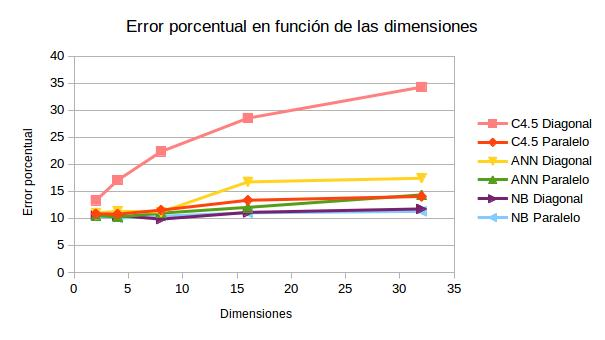
\includegraphics[scale=0.8]{ejercicio2}
	\caption{Error porcentual en función de las dimensiones para gaussianas diagonales y paralelas, utilizando todos los clasificadores vistos hasta ahora.}
\end{figure}

\bigskip

A partir de la Figura 1, se puede notar que el menor error porcentual es obtenido utilizando el clasificador mencionado anteriormente. A su vez, no se presentan diferencias para los datos paralelos y diagonales. Todo esto es de esperar ya que, justamente, el modelo que toma este algoritmo es una gaussiana. A continuación se presentan los valores que toman las medias y las desviaciones estándares para gaussianas diagonales y paralelas de dos dimensiones.

\newpage

 \begin{verbatim}
 Gausiana Diagonal - 2 dimensiones 
 Clase 0 Atributo 0 Media: -1.032835 DE: 1.132444
 Clase 0 Atributo 1 Media: -0.934291 DE: 1.288594
 Clase 1 Atributo 0 Media: 0.988550 DE: 1.121291
 Clase 1 Atributo 1 Media: 0.978897 DE: 1.121600
 
 
\end{verbatim}

\begin{verbatim}
 Gausiana Paralela - 2 dimensiones
 Clase 0 Atributo 0 Media: 0.944522 DE: 0.782636
 Clase 0 Atributo 1 Media: -0.024705 DE: 0.786007
 Clase 1 Atributo 0 Media: -0.947048 DE: 0.813101
 Clase 1 Atributo 1 Media: 0.083738 DE: 0.772095 
 \end{verbatim}
Recordemos que las gaussianas diagonales de 2 dimensiones tienen medias de (-1,-1) y (1,1) y desviaciones estándares de aproximadamente 1.1, y las paralelas, medias de (1,0) y (-1,0) y desviaciones estándares de 0.78. Si se comparan los valores reales con los calculados por el algoritmo, se puede deducir que encuentra muy bien las dos gaussianas. \\
Si se observan los resultados, por ejemplo, para 32 dimensiones, se nota que para algunos atributos no estima tan bien la media. De igual modo con la desviación estándar. Sin embargo, el error porcentual para esta cantidad de dimensiones es similar al error porcentual para dos dimensiones (según la Figura 1). Por lo tanto, se puede concluír que el algoritmo funciona bien aún con muchas dimensiones.

\section*{Ejercicio 3}

En este ejercicio se pide resolver los problemas de espirales anidadas y dos elipses con el algoritmo de Naive Bayes con Gaussianas. Dado que este algoritmo utiliza un modelo de distribución normal para hacer las predicciones de las clases, y considerando que ninguno de estos problemas responde a una gaussiana, es esperable que se encuentren malos resultados.

\bigskip

En la Figura 2 se grafican las predicciones para el conjunto de test para ambos problemas.

\begin{figure}
    \centering

    \begin{subfigure}[b]{0.45\textwidth}
        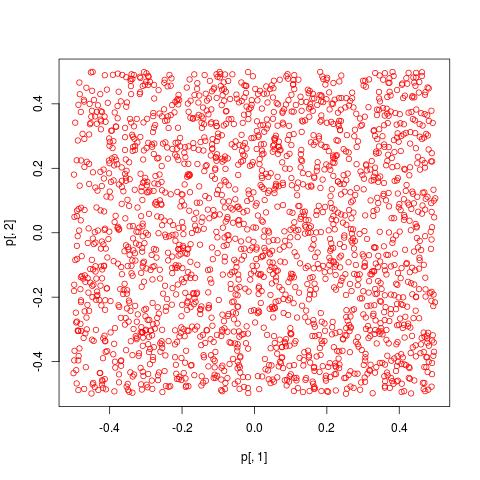
\includegraphics[width=\textwidth]{doselipses1}
        \caption{Conjunto de datos dos elipses}
        %\label{fig:tiger}
    \end{subfigure}
      ~ %add desired spacing between images, e. g. ~, \quad, \qquad, \hfill etc. 
      %(or a blank line to force the subfigure onto a new line)
    \begin{subfigure}[b]{0.45\textwidth}
        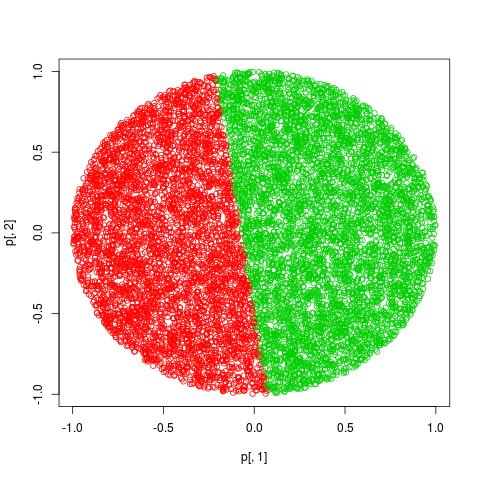
\includegraphics[width=\textwidth]{espirales1}
        \caption{Conjunto de datos espirales anidadas}
        %\label{fig:gull}
    \end{subfigure}
    \caption{Predicciones para el conjunto de test utilizando el clasificador  Naive Bayes con Gaussianas. }
\end{figure}

\subsection*{Dos elipses}
 El error porcentual en test para dos elipses es del 24.35 \%. Esto es así porque clasifica todos los puntos como puntos de la clase 0. A continuación se muestran los cálculos de las medias y las desviaciones estándares que realiza el algoritmo, por clase y por atributo. Los cálculos divididos por atributos se deben a que considera que cada dimensión es independiente de la otra.

\newpage
\begin{verbatim}
DOS ELIPSES
 Clase 0 Atributo 0 Media: -0.001270 DE: 0.308843
 Clase 0 Atributo 1 Media: -0.001872 DE: 0.325014
 Clase 1 Atributo 0 Media: -0.015273 DE: 0.262829
 Clase 1 Atributo 1 Media: -0.001733 DE: 0.129106
\end{verbatim}

Allí vemos que para ambas clases encuentra distribuciones normales con aproximadamente la misma media. La desviación estándar es mayor para la clase 0 que para la 1, lo cual es razonable, siendo que los puntos de la clase 0 tienen mayor distancia máxima del (0,0) tanto por el eje X como por el eje Y,\footnote{Recordar que este algoritmo no utiliza distancias euclidianas, ya que considera a todas las variables independientes.} que los puntos de clase 1. A su vez. la desviación estándar es mayor para la clase 1, atributo 0 (eje X), que para el atributo 1 (eje Y). Esta decisión también parece tener sentido ya que la distancia en el eje Y desde el 0, hasta el punto más lejano de clase 1, es aproximadamente 0.2. De distinta manera, para el eje X, la distancia desde el 0, hasta el punto más lejano, es aproximadamente 0.4. Esto se puede observar en la Figura 3.\\
Considerando que las gausianas para ambas clases se encuentran encimadas y que la probabilidad a priori juega a favor de la clase 0 (0.75 de probabilidad frente a 0.25), parece ser compresnible la clasificación del algoritmo.

\begin{figure}
    \centering
	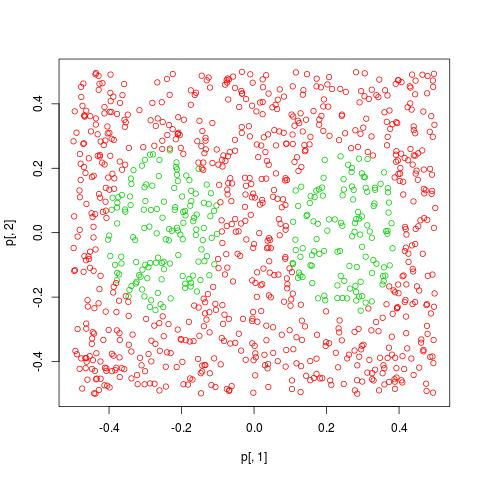
\includegraphics[scale=0.45]{dos_elipses}
	\caption{Conjunto data de 1000 puntos para el problema de las dos elipses. 250 puntos pertenecen a la clase 1 (verde), y 750 a la 0 (roja).}
\end{figure}

\bigskip

\subsection*{Espirales anidadas}
El error porcentual en test para las espirales anidadas es de aproximadamente el 43\%, según la ejecución. A continuación se presenta un ejemplo de los valores que toman las medias y las desviaciones estándares, por clase y por atributo. 

\begin{verbatim}
ESPIRALES ANIDADAS
 Clase 0 Atributo 0 Media: -0.118910 DE: 0.499409
 Clase 0 Atributo 1 Media: -0.033010 DE: 0.502357
 Clase 1 Atributo 0 Media: 0.079960 DE: 0.477544
 Clase 1 Atributo 1 Media: -0.001972 DE: 0.502946
\end{verbatim}
Allí se puede observar que se está estimando prácticamente la misma gausiana para cada clase y para cada atributo. Todas las distribuciones normales tienen una media muy cercana a 0, y una desviación estándar similar a 0.5. Sin embargo, si se observan las medias asignadas por clase para el atributo 0 (X), se puede ver que el valor elegido para la 0 (roja) se encuentra más a la izquierda que su contraparte para la clase 1 (verde). Una posible explicación para ésto se puede deducir si se mira con detenemiento la gráfica del conjunto de entrenamiento utilizado, presentado en la Figura 4. Si se divide dicho conjunto de puntos a través de un segmento paralelo al eje Y que pasa por el (0,0), entonces a la derecha quedarán más puntos verdes que rojos, y a la izquierda, más rojos que verde. Esto explica las tendencias de los corrimientos de la media para el atributo X respecto al centro del eje, y justifica la clasificación de los puntos observada en la Figura 2.

\begin{figure}
    \centering
	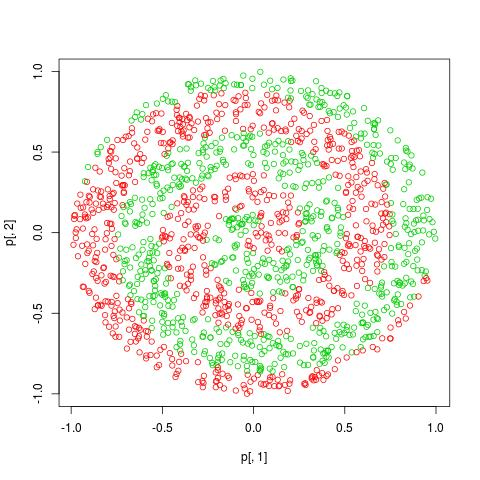
\includegraphics[scale=0.35]{espirales}
	\caption{Conjunto data de 1500 puntos para el problema de las dos elipses. 750 puntos pertenecen a la clase 1 (verde), y 750 a la 0 (roja).}
\end{figure}

\section*{Ejercicio 4}

En este ejercicio se pide implementar el clasificador Naive Bayes con Histogramas. A diferencia del algoritmo anterior, en este caso, la probabilidad P(a$|$C), siendo \textit{a} un valor para el atributo \textit{i}, y \textit{C} una clase, se aproxima calculando la frecuencia en que el atributo \textit{i} toma el valor \textit{a}, siendo de la clase \textit{C}. El código correspondiente se encuentra en el archivo \textit{ejercicio4.c}.

\subsection*{Dos elipses}

El experimento se realizó variando la cantidad de bins entre los valores 1, 2, 5, 8, 10, 12, 15, 20, 25, 30, 50, 70, 100, 200, 300 y 1000. En la Figura 5 se muestra el error porcentual de entrenamiento, validación y test en función de la cantidad de bins para dicho problema. Allí se puede observar que a medida que aumenta la cantidad de bins, el error de test y de validación tienden a crecer. En la Figura 3 (b) se puede apreciar que, a partir de aproximadamente 30 bins, el error de entrenamiento comienza a bajar, mientras que el de test y de validación, a subir. Esto es un claro índice de que se está haciendo sobreajuste.

\begin{figure}
    \centering

    \begin{subfigure}[b]{0.45\textwidth}
        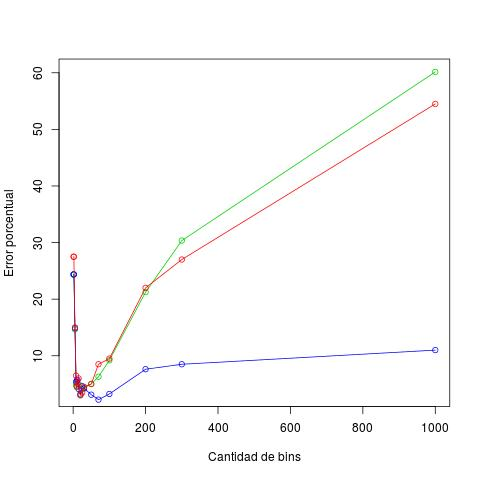
\includegraphics[width=\textwidth]{errorde}
        \caption{Utilizando todos los bins}
        %\label{fig:tiger}
    \end{subfigure}
      ~ %add desired spacing between images, e. g. ~, \quad, \qquad, \hfill etc. 
      %(or a blank line to force the subfigure onto a new line)
    \begin{subfigure}[b]{0.45\textwidth}
        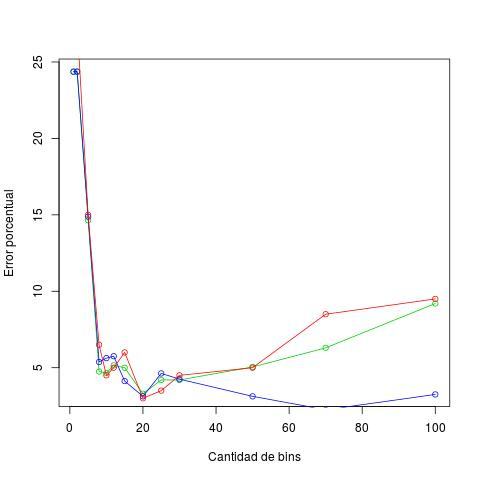
\includegraphics[width=\textwidth]{errorde2}
        \caption{Utilizando bins menores a 100}
        %\label{fig:gull}
    \end{subfigure}
    \caption{Error porcentual en test, entrenamiento y validación en función de los bins. Las curvas azules corresponden al entrenamiento, las verdes al test, y las rojas, a la validación}
\end{figure}

\bigskip

Para analizar de dónde proviene este sobreajuste primero vamos a analizar un poco el conjunto de entrenamiento que se está utilizando. En la Figura 3 se graficaron los mil puntos que contiene el conjunto data. Sin embargo, para este caso, estamos utilizando 800 puntos para entrenar y 200 para validar. Si se observa dicha gráfica, se puede notar que los puntos suelen estar espaciados, y que existen huecos relativamente grandes en algunos sectores. \\
A su vez, en el conjunto data existen 750 puntos de clase 0 y 250 de clase 1. Dado que el cojunto de entrenamiento es elegido al azar, es esperable que la proporción entre puntos de ambas clases se mantenga.


\bigskip

Otra cuestión a tener en cuenta para entender por qué hay sobreajuste es la forma en la cual se están generando los histogramas. Por un lado, la cantidad de bins es tomada como parámetro de entrada, y cada bin para un atributo dado, tiene el mismo ancho. A su vez, se está usando una estimación de la probabilidad, para evitar casos en los cuales la frecuencia de un punto con características particulares es cero. Por esto se utiliza una constante \textit{m}, denominada \textit{equivalent sample size}, y la probabilidad P(a$|$C) para la dimensión \textit{i}, se calcula como $\dfrac{n_{a} + 1} {n + m}$, donde \textit{$n_{a}$} es la cantidad de puntos con clase \textit{C}, cuya dimensión \textit{i} pertenece al mismo bin que el valor \textit{a}, \textit{n} es la cantidad de puntos de de clase \textit{C}, y \textit{m} es la constante nombrada anteriormente.\\
En nuestro experimento se tomó un valor de \textit{m} igual a 1, por lo tanto nuestro cálculo de la probabilidad se reduce a $\dfrac{n_{a} + 1} {n + 1}$.\\
¿Qué ocurre cuando crece la cantidad de bins? Pensemos que mientras mayor cantidad de bins haya, éstos serán de ancho menor, y por lo tanto los valores entre los que debe estar un atributo dado para pertenecer a ese bin serán más cercanos. De éste modo, cada vez habrá más cantidad de bins con pocos o cero puntos, y en consecuencia, el valor de \textit{$n_{a}$} tenderá a bajar. Finalmente, al calcular las probabilidades para cada clase, se encontrará que será más probable la clase a la cual pertenezcan menos puntos. De este modo se \textquotedblleft beneficia\textquotedblright a la clase 1 (verde en la gráfica).\\
Este análisis justifca el hecho de que, a mayor cantidad de bins, hay mayor error porcentual en test y en validación.

\begin{figure}
    \centering

    \begin{subfigure}[b]{0.42\textwidth}
        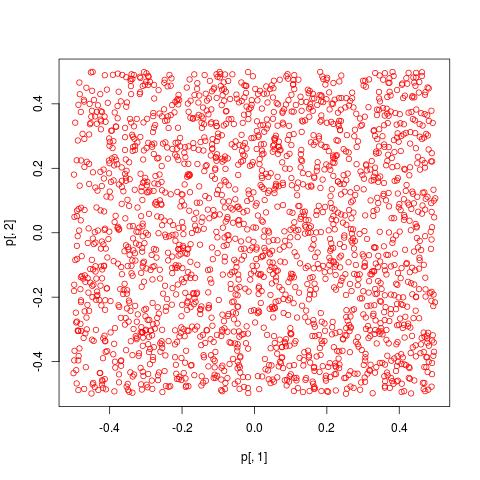
\includegraphics[width=\textwidth]{prediccion2}
        \caption{2 bins}
        %\label{fig:tiger}
    \end{subfigure}
      ~ %add desired spacing between images, e. g. ~, \quad, \qquad, \hfill etc. 
      %(or a blank line to force the subfigure onto a new line)
    \begin{subfigure}[b]{0.42\textwidth}
        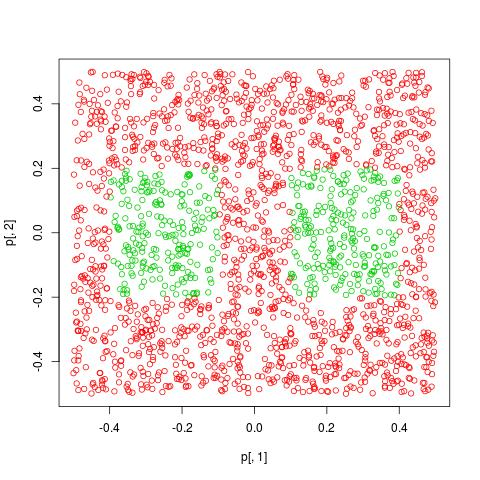
\includegraphics[width=\textwidth]{prediccion5}
        \caption{10 bins}
        %\label{fig:gull}
    \end{subfigure}
    ~ %add desired spacing between images, e. g. ~, \quad, \qquad, \hfill etc. 
      %(or a blank line to force the subfigure onto a new line)
    \begin{subfigure}[b]{0.42\textwidth}
        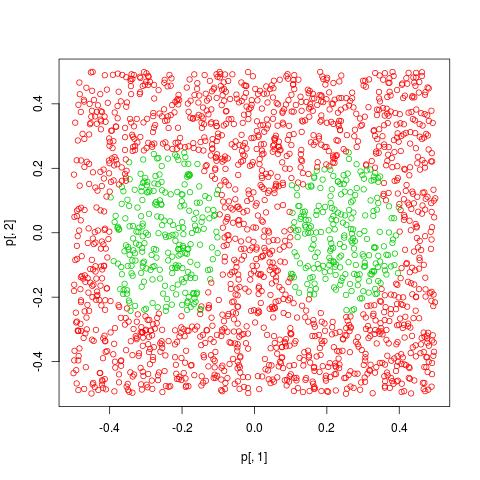
\includegraphics[width=\textwidth]{prediccion8}
        \caption{20 bins}
        %\label{fig:tiger}
    \end{subfigure}
    \begin{subfigure}[b]{0.42\textwidth}
        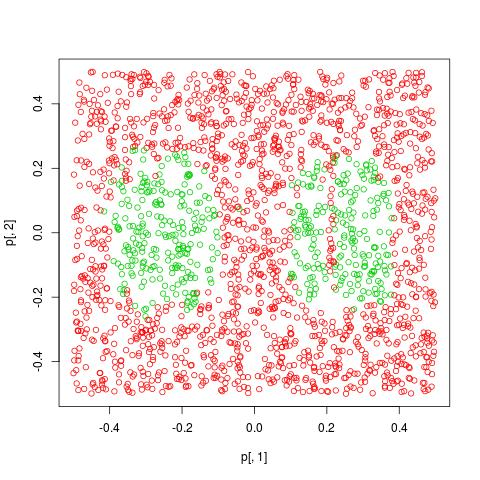
\includegraphics[width=\textwidth]{prediccion11}
        \caption{50 bins}
        %\label{fig:tiger}
    \end{subfigure}
      ~ %add desired spacing between images, e. g. ~, \quad, \qquad, \hfill etc. 
      %(or a blank line to force the subfigure onto a new line)
    \begin{subfigure}[b]{0.42\textwidth}
        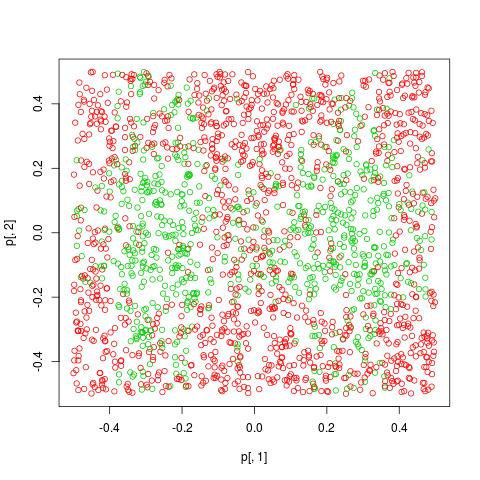
\includegraphics[width=\textwidth]{prediccion14}
        \caption{200 bins}
        %\label{fig:gull}
    \end{subfigure}
    ~ %add desired spacing between images, e. g. ~, \quad, \qquad, \hfill etc. 
      %(or a blank line to force the subfigure onto a new line)
    \begin{subfigure}[b]{0.42\textwidth}
        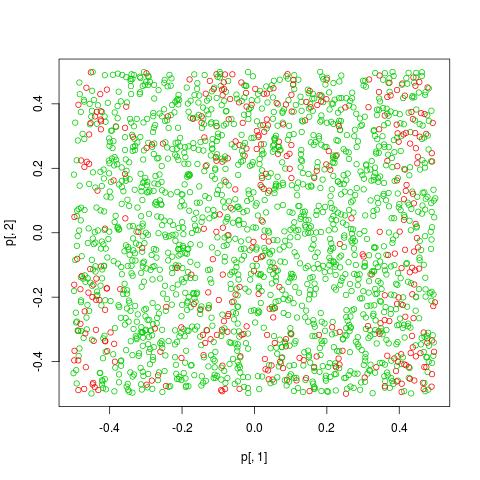
\includegraphics[width=\textwidth]{prediccion16}
        \caption{1000 bins}
        %\label{fig:tiger}
    \end{subfigure}    
    \caption{Predicciones para el problema de las dos elipses, utilizando el clasificador Naive Bayes con Histogramas.}
\end{figure}


\bigskip

En la Figura 6 se grafican las predicciones variando la cantidad de bins utilizados. Allí se puede observar lo analizado anteriormente. Para un número de bins igual a 2, toda la predicción pertenece a la clase mayoritaria, lo cual es muy razonable. Si se divide la gráfica a la mitad tanto en X como en Y, es esperable que siempre sea más probable que el punto sea de clase 0.  \\
La gráfica correspondiente a 10 bins, empieza a mostrar los dos sectores en donde los puntos son verdes, pero la cantidad de bins no alcanza para que se vean las terminaciones redondeadas de las elipses. Es por esto que se ven dos rectángulos.\\
Cuando se utilizan 20 bins, se obtiene la predicción óptima para este problema. Esto se puede ver en la gráfica de errores porcentuales.  Posiblemente, esta cantidad de bins sea suficiente para que se aprecien las terminaciones redondeadas de las elipses, pero no sea tan pequeña como para que empiecen a quedar bins vacíos o con muy pocos puntos.\\
En la Figura 6 (d) se observa que en la elipse de la derecha aparece una línea de puntos rojos. Esto posiblemente sea producido proque en el conjunto de entrenamiento existe un hueco en ese sector, y por lo tanto el bin correspondiente queda principalmente con puntos rojos. Esto es un primer indicio de que los bins comienzan a ser excesivamente pequeños.\\
Si se observan las siguientes gráficas, la tendencia de tener bins vacíos aumenta con la cantidad de éstos y la clase verde se expande por completo (Figura 6 (e) y (f)).

\bigskip

Si se comparan estos resultados con los obtenidos en el Ejercicio 3, utilizando el clasificador Naive Bayes con Gaussianas, se puede concluír para un problema con características como el de las dos elipses, es mejor utilizar un modelo basado en histogramas.

\subsection*{Espirales anidadas}
Análogamente, para este nuevo problema, se graficaron los error porcentuales en test, entrenamiento y validación en función de la cantidad de bins. Esto se puede encontrar en la Figura 7. Nuevamente, se puede observar que a partir de 30 bins, se empieza a apreciar el sobreajuste. Sin embargo, los errores porcentuales en test nunca bajan del 25\%, manteniéndose en el órden del 30\%. Para analizar por qué ocurre esto, es conveniente observar con detenemiento el conjunto de entrenamiento utilizado.

\begin{figure}
    \centering

    \begin{subfigure}[b]{0.45\textwidth}
        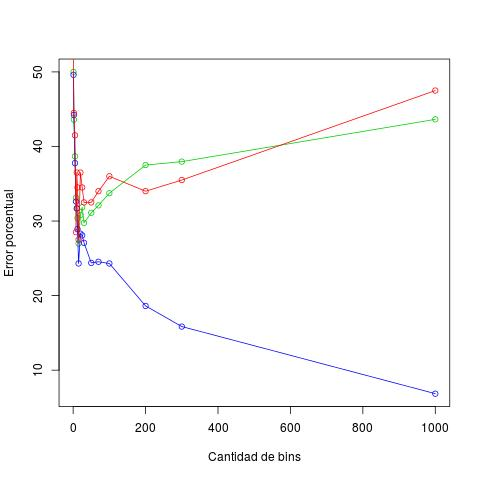
\includegraphics[width=\textwidth]{errorea}
        \caption{Utilizando todos los bins}
        %\label{fig:tiger}
    \end{subfigure}
      ~ %add desired spacing between images, e. g. ~, \quad, \qquad, \hfill etc. 
      %(or a blank line to force the subfigure onto a new line)
    \begin{subfigure}[b]{0.45\textwidth}
        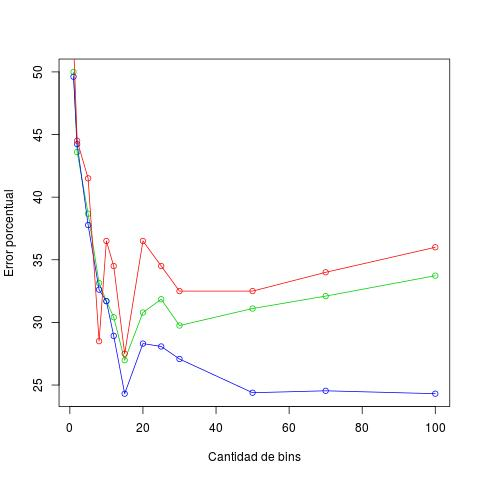
\includegraphics[width=\textwidth]{errorea2}
        \caption{Utilizando bins menores a 100}
        %\label{fig:gull}
    \end{subfigure}
    \caption{Error porcentual en test, entrenamiento y validación en función de los bins. Las curvas azules corresponden al entrenamiento, las verdes al test, y las rojas, a la validación}
\end{figure}

\bigskip

En la Figura 4 se graficaron los 1500 puntos del archivo data para el problema de las espirales anidadas. En dicho conjunto existen 750 puntos de clase 0 (roja) y 750 puntos de clase 1 (verde). Para entrenar se utilizaron 1300 puntos tomados al azar. Por lo tanto, es esperable la relación 50\%50\% se mantenga. Por este motivo, las probabilidades a priori no deben ser tenidas en cuenta en este problema, ya que sería razonable que fueran muy similares para ambas clases.

\bigskip

Ahora bien, ¿cuál es la diferencia entre el problema de las espirales anidadas y el de dos elipses? ¿Por qué uno puede ser resuelto por el clasificador y el otro no? La clave está en pensar cómo están los puntos distribuídos en el plano, según la clase. Para el problema de las dos elipses, los puntos de una misma clase se encuentran compactos, agrupados de manera tal que las clases se pueden dividir trazando líneas paralelas al eje X y al eje Y de manera aceptablemente correcta. Esta idea se puede observar en la Figura 8 (c). Sin embargo, no es suficiente con aquello para que el problema pueda ser resuelto por el clasificador utilizado.\footnote{Pensar que si eso fuera condición suficiente, este clasificador sería capaz de resolver el problema XOR perfectamente, cuando en realidad no lo puede hacer. De hecho, es la peor clase de problema posible para este algoritmo.} La cuestión fundamental es que si se toma un punto cualquiera del cual se quiere predecir la clase, hacerlo en función de la cantidad de puntos de cada clase que hay en cada uno de los dos bins a los cuales pertenece (uno por el atributo X, y otro por el atributo Y), tiene mucho sentido.\\
A modo de visualizar mejor esta idea, en la Figura 8 (a) y (b) se muestran ejemplos de los cuadrantes que son tenidos en cuenta para determinar la clase de un punto dado. El punto cuya clase se desea determinar y los cuadrantes tenidos en cuenta se marcan en violeta. Notar que el cuadrante al cual pertenece el punto, se considera dos veces, ya que pertenece a ambos bins.\\
Es decir, este algoritmo, utiliza una medida de distancia que considera a las variables por separado. Por lo tanto, dos puntos que tienen valores similares para un atributo dado, son considerados cercanos cuando se evalúa dicha dimensión. Esto no puede ser utilizado para resolver el problema de las espirales anidadas, ya que en ese conjunto de datos, a lo largo de los bins (puntos \textit{parecidos} para el algoritmo), en general, hay tantos puntos verdes como rojos.
\begin{figure}
    \centering
      ~ %add desired spacing between images, e. g. ~, \quad, \qquad, \hfill etc. 
      %(or a blank line to force the subfigure onto a new line)
    \begin{subfigure}[b]{0.35\textwidth}
        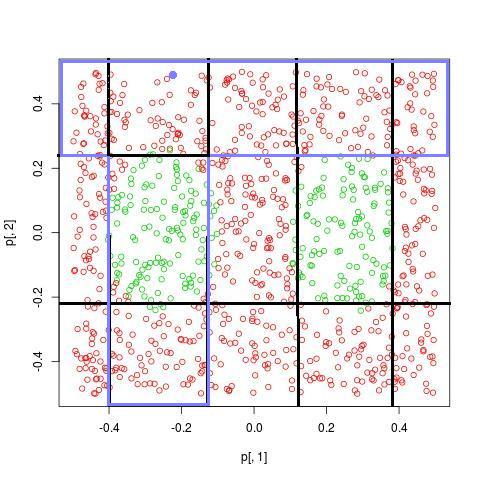
\includegraphics[width=\textwidth]{dos_elipses_ej1}
        \caption{Ejemplo de puntos tenidos en cuenta para la determinación de la clase}
        %\label{fig:gull}
    \end{subfigure}
    \begin{subfigure}[b]{0.35\textwidth}
        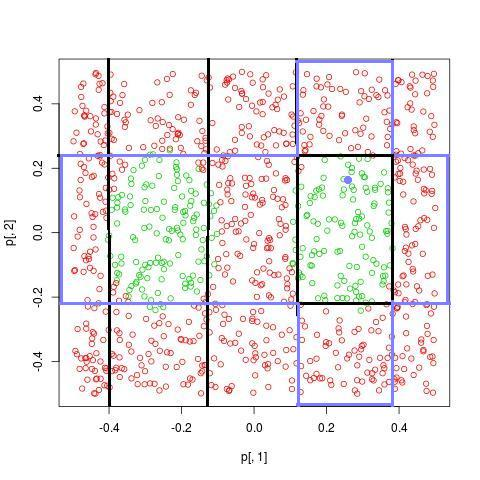
\includegraphics[width=\textwidth]{dos_elipses_ej2}
        \caption{Ejemplo de puntos tenidos en cuenta para la determinación de la clase}
        %\label{fig:gull}
    \end{subfigure}  
    \begin{subfigure}[b]{0.35\textwidth}
        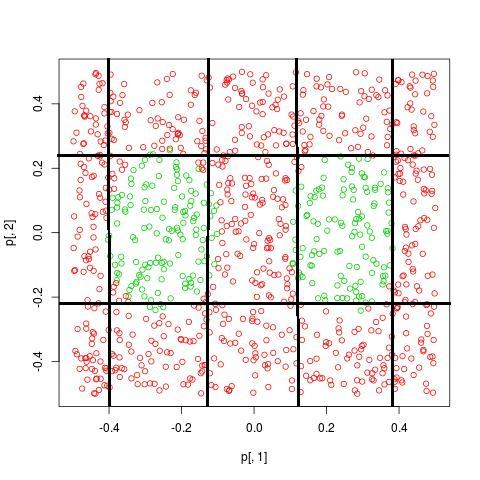
\includegraphics[width=\textwidth]{dos_elipses_cuadrantes}
        \caption{División en cuadrantes para el problema de las dos elipses}
        %\label{fig:tiger}
    \end{subfigure}      
    \caption{}
\end{figure}

\bigskip

En la Figura 9 se grafican las predicciones obtenidas para las espirales anidadas, aumentando la cantidad de bins. Allí se observa que ninguna clasificación resuelve el problema.

\begin{figure}
    \centering
      ~ %add desired spacing between images, e. g. ~, \quad, \qquad, \hfill etc. 
      %(or a blank line to force the subfigure onto a new line)
    \begin{subfigure}[b]{0.40\textwidth}
        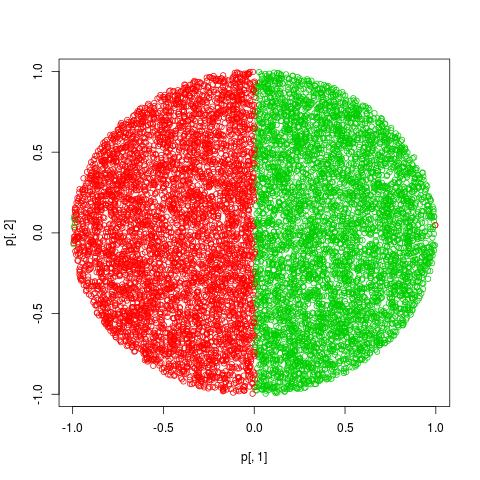
\includegraphics[width=\textwidth]{prediccion2ea}
        \caption{2 bins}
        %\label{fig:gull}
    \end{subfigure}
    \begin{subfigure}[b]{0.40\textwidth}
        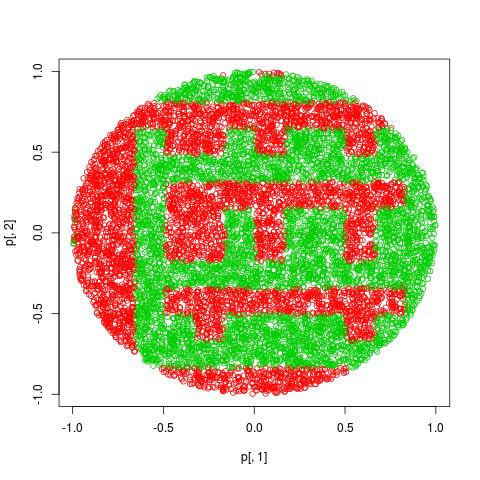
\includegraphics[width=\textwidth]{prediccion6ea}
        \caption{12 bins}
        %\label{fig:gull}
    \end{subfigure}  
    \begin{subfigure}[b]{0.40\textwidth}
        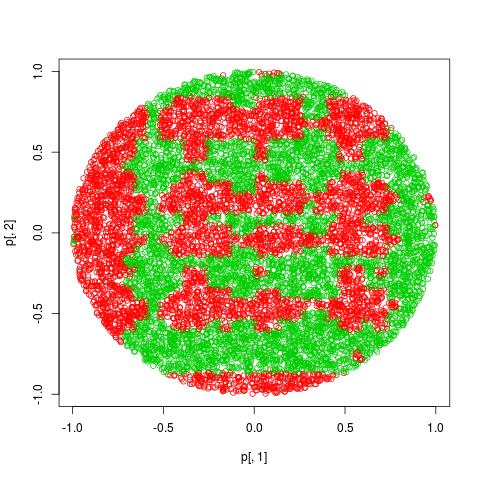
\includegraphics[width=\textwidth]{prediccion10ea}
        \caption{30 bins}
        %\label{fig:tiger}
    \end{subfigure}      
        \begin{subfigure}[b]{0.40\textwidth}
        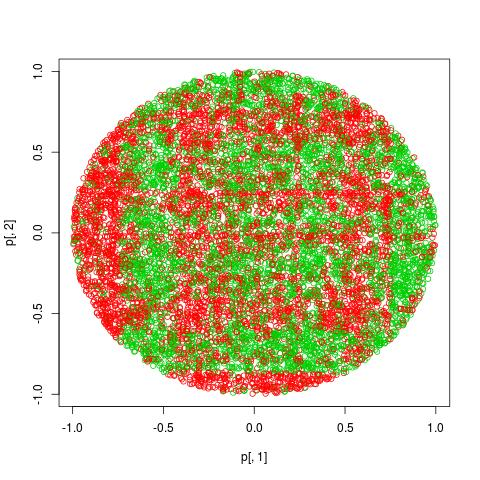
\includegraphics[width=\textwidth]{prediccion15ea}
        \caption{300}
        %\label{fig:tiger}
    \end{subfigure}      
    \caption{Predicciones obtenidas con el clasificador Naive Bayes con Histogramas para las espirales anidadas}
\end{figure}

\bigskip

Si se comparan estos resultados con los obtenidos al utilizar el clasificador Naive Bayes con Gaussianas, se puede concluír que, si bien el modelo con histogramas presenta mejores resultados, ninguno de éstos algoritmos es capaz de resolver este problema.

\section*{Ejercicio 5}
En este ejercicio se pide implementar un clasificador Naive Bayes con Histogramas, en el cual los atributos no son considerados independientes, y resolver el problema de las espirales anidadas. Este algoritmo es similar al anterior, a diferencia que en lugar de considerar bins para cada atributo por separado, limita todos los atributos a ciertos valores al mismo tiempo. La cantidad \textit{b} de bins para cada atributo se toma como parámetro de entrada, y luego, se clasifican los puntos en $\textit{b}^{a}$ grupos, donde \textit{a} es la cantidad de atributos. Finalmente, para definir la clase de una nueva instancia, el algoritmo busca el casillero al cual pertenece según los valores que toman los atributos, y elige la clase más probable para ese conjunto. El código correspondiente se encuentra en el archivo \textit{ejercicio5.c}.

\bigskip

Si bien este algoritmo parece a primera vista capaz de resolver cualquier clasificación, tiene un problema fundamental: su complejidad es del orden de \textit{n}$\textit{b}^{a}$, donde \textit{n} es la cantidad de puntos de entrenamiento, \textit{b} la cantidad de bins, y \textit{a} el número de atributos. Por lo tanto, se hace inmanejable para conjuntos de datos de muchas variables.

\bigskip

En cuanto a la resolución del problema de las espirales anidadas con este algoritmo, es esperable que se logre una buena clasificación, para una cantidad razonable de bins. Por un razonamiento análogo al hecho para el clasificador del Ejercicio 4, un número excesivo de bins produce sobreajuste. La mejor clasificación encontrada fue la que se realizó utilizando 16 bins, presentando menos del 10\% de error en test. Se grafica en la Figura 10.\\
Naturalmente, se observan terminaciones rectas, porque los bins no son lo suficientemente pequeños como para suavizar las curvas. Sin embargo, esto no se puede evitar, ya que si se aumenta la cantidad de bins, aparece el sobreajuste. Este tipo de predicción recuerda a las que se obtuvieron con los árboles de decisión.

\begin{figure}
    \centering
	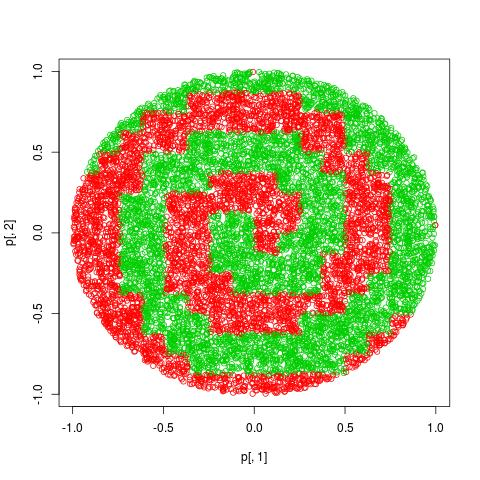
\includegraphics[scale=0.45]{espiralesInd}
	\caption{Predicciones para el conjunto de espirales anidadas utilizando el clasificador Naive Bayes con Histograma sin considerar las variables independientes, utilizando 16 bins.}
\end{figure}


\section*{Ejercicio 6}
En este ejercico se pide implementar el algoritmo de discretización recursiva por mínima entropía. La principal característica de dicho clasificador es que define, a partir de cálculos de entropía de conjuntos, la cantidad de bins por atributo, y a su vez, el ancho de cada uno. El código correspondiente se encuentra en el archivo \textit{ejercicio6.c}.

\bigskip

Al resolver el problema de las dos elipses con este clasificador, es esperable que arme bins similares a los presentados en la Figura 8 (c). Siendo que el algoritmo considera cada variable independiente, los bins siempre definen límites para un atributo en particular, y no importa qué valor toma el punto para las otras dimensiones.\\
Los cortes que hace el algoritmo son los siguientes:
\begin{verbatim}
X: -0.402618 -0.156555 -0.099243 0.106232 0.382355 
Y: -0.242188 0.152832 0.244263 
\end{verbatim}
En la Figura 11 se presenta el conjunto de entrenamiento para dos elipses con los bins que elige el algoritmo en cuestión. Allí se observa que define los bins esperados, agregando un bin extra para cada atributo. 

\begin{figure}
    \centering
	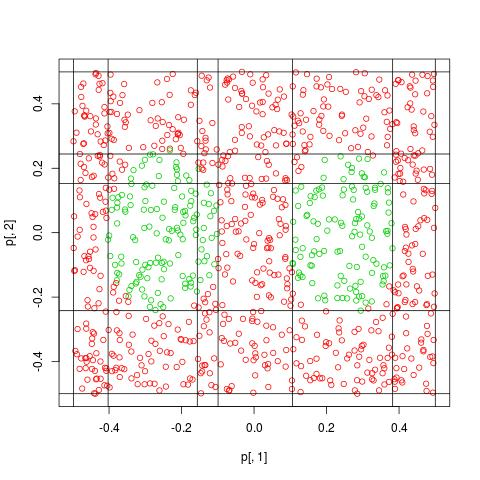
\includegraphics[scale=0.45]{ej6bins}
	\caption{Bins definidos por el algoritmo de discretización recursiva por mínima entropía para el conjunto de entrenamiento de dos elipses.}
\end{figure}

El error obtenido en test con este algoritmo es de 4.1\%, similar al mejor obtenido con el algoritmo Naive Bayes con Histogramas. Sin embargo, este clasificador tiene la ventaja de que no hace falta hacer un barrido con la cantidad de bins, ya que ésto lo determina el mismo algoritmo. A su vez, se evita el riesgo de sobreajuste, y el hecho de que los bins puedan ser de distinto ancho, hace que la predicción sea más precisa con menor cantidad de bins. Dicha predicción se grafica en la Figura 12.

\begin{figure}
    \centering
	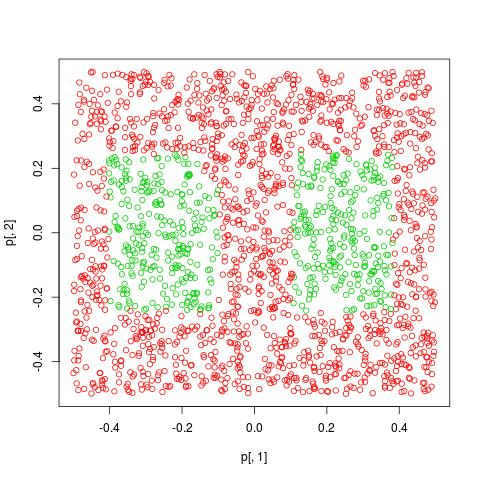
\includegraphics[scale=0.45]{dos_elipses_6}
	\caption{Predicción para dos elipses obtenida con el clasificador de discretización recursiva por mínima entropía.}
\end{figure}





\end{document}